\documentclass[12pt,
	parskip=half,		% Abstände statt Einrückungen bei Absätzen
	department=FakEI,  	% Farbanpassungen
	oneside, 			% Spart Papier und erhöht die Lesbarkeit
	DIV=15,BCOR=10mm, 	% Seitenlayout wie bei Koma-Script
	svgnames,table, 	% Optionen für xcolor
	useDepartmentLogo,  % mit Logo der Fakultät
	bookmarks, raiselinks, pageanchor, hyperindex, colorlinks, hidelinks, % Optionen für hyperref
]{OTHRreprt}

% Encoding ist UTF-8
\usepackage[utf8x]{inputenc}

% Sprache ist Deutsch bzw. Englisch
\usepackage[english,ngerman]{babel}

% Formateinstellungen Links (Extern: Blau, Intern: Schwarz)
\usepackage[colorlinks=true,linkcolor=red, urlcolor=blue]{hyperref}

% Einstellungen für Kopf bzw. Fußzeile
\usepackage[automark,headsepline=.4pt,plainheadsepline]{scrlayer-scrpage}         % Erstellung von selbst definierten Kopfzeilen
\clearpairofpagestyles%\clearscrheadfoot veraltet
\renewcommand{\chaptermarkformat}{}
\setkomafont{pageheadfoot}{\normalfont}
\automark*{chapter}

% Kopfzeile
\ohead*{\pagemark}
\ihead*{\leftmark}

% Fußzeile
\cfoot*{\pagemark}
\makeatletter
\ofoot*{\@author}
\makeatother

% Einstellungen/package das für Abkürzungen genutzt wird.
\usepackage{acronym}

% Anführungszeichen sollen aus dem Deutschen verwendet werden.
\usepackage[autostyle=true,german=quotes]{csquotes}

% Mathematik pakete
\usepackage{amsmath}
\usepackage{siunitx}
\sisetup{locale = DE}

% Bilder
\usepackage{wrapfig}
\usepackage{graphicx}
\graphicspath{{images/}}

% Tikz
\usepackage{tikz}
\usetikzlibrary{arrows,positioning, calc, shapes.misc, decorations.markings}

% Quellen
\bibliographystyle{plain}

% Tabellen
\usepackage{tabularx}
\usepackage{booktabs}

% Listen
\usepackage{enumitem}
\setlist{itemsep=-0.5ex, topsep=0pt}

% Captions
\usepackage{caption}
% \captionsetup{font=bf} % Einkommmentieren für Fettgedruckte Captions

% Sonstiges
\usepackage[most]{tcolorbox} % Schöne farbboxen
\usepackage{fontawesome} % Bilder aus dem fontawesome set.

% Metadaten des Dokuments
\documenttype{Projektarbeit}
\title{FPGA basierter BPSK/QPSK Empfänger}
\date{22.02.2024}

\author{Hannes Bachl}
\studentid{3321274}

\studyprogramme{Bachelor Elektro- und Informationstechnik}
\department{Elektro- und Informationstechnik}
\firstadvisor{Prof. Dr.-Ing. Florian Aschauer}


\makeatletter
\hypersetup{pdftitle={\@title},%
	pdfauthor={\@author},%
}
\makeatother

% Selbst definierte macro für dieses Script
\usepackage{macros}

% ================================ START Konfiguration ================================

% ================================ ENDE Konfiguratiobn ================================

\begin{document}
	\pagenumbering{Roman}	
	
	% Titleseite
	\maketitle
	
	% Arbeite wurde Selbsterstellt.
	\makedeclaration
	
	% Abstract
	\begin{abstract}
		% Input wird benutzt, damit keine leeren Seiten davor bzw. dahinter entstehen.
		\begin{quote}

	\section*{Vorwort}
	Inhalt dieser Projektarbeit ist die Erstellung eines einfachen \acl{SDR} zum Empfang eines \acs{QPSK} oder \acs{BPSK} modulierten Signales.
	Als Basis kommt hier ein \acl{FPGA} mit angeschlossenem externen \acl{ADC} zum Einsatz.\\
	
	Hauptaugenmerk soll dabei auf der eigenen Umsetzung der für ein \acs{SDR} notwendigen Signalverarbeitungsalgorithmen sowie den Kommunikationsstrukturen, welche
	benötigt werden um einer \acl{CPU} die Steuerung der umgesetzten Schaltung zu ermöglichen, liegen.

	Das Projekt soll als grundlegende Basis für, ein eventuell später noch umzusetzendes, komplexeres \acs{SDR} dienen und ist deswegen, wo möglich,
	flexibel gestaltet.

\end{quote}
	
	\end{abstract}
	
	% Inhaltsverzeichniss
	\tableofcontents
	\cleardoublepage
	% Inhalt
	\pagenumbering{arabic}	
	
	\chapter{Einleitung}
Inhalt dieses Projektes ist die Erstellung eines \acs{SDR}, wobei ein \acs{FPGA} als Plattform dienen soll. 
Der \acs{FPGA}-Logikteil soll weiterhin von einem Rechenkern, für die weitere Datenverarbeitung, unterstützt werden.

Da es sich um ein Lernprojekt handelt soll der Fokus, bei der Erstellung der \acs{FPGA}-Schaltung, auf der selbständigen Erstellung aller Signal verarbeitenden Blöcke liegen.
Komplexe Blöcke welche für die Kommunikation mit dem Rechensystem benötigt wurden \textit{(z.B. AXI-Infrastruktur)} wurden aus Zeitgründen nicht selbst erstellt, sondern das vorhandene
IP des \acs{FPGA}-Herstellers verwendet.

\section{Anforderungen}
Zu beginn des Projektes wurde mit der Festlegung der Anforderungen an des Gesamtsystem begonnen, um so die notwendigen Hardware- und Logikkomponenten richtig auslegen zu können.

Dabei wurden die folgende Anforderungen an das System definiert:
\begin{enumerate}
	\item \textbf{Unterstützung der Verwendung eines extern \acs{ADC}}
	\begin{enumerate}[label*=\arabic*.]
		\item Abtastfrequenz von mindestens \qty{100}{M\hertz} [$f_{ADC} > \qty{100}{M\hertz}$].
		\item Datenbreite soll mindestens \qty{12}{bit} betragen [$w_{adc} > 12$]
		\item Externer anti-Alias Filter notwendig und Abtastung in der ersten Nyquist-Zone.
	\end{enumerate}

	\item \textbf{Digitale Abwärtsmischung in das Basisband}
	\begin{enumerate}[label*=\arabic*.]
		\item Eingangssignal im Frequenzbereich \qty{1}{M\hertz} bis \qty{20}{M\hertz}. [$f_s \in [\qty{1}{M\hertz};\qty{20}{M\hertz}]$]
		\item Interner \acl{NCO} wobei die Frequenz im Frequenzbereich variable verstellbar sein soll
		\item Interner komplexer Mischer mit $\qty{16}{bit}$-Breitem $I/Q$ Signal am Ausgang
		\item Dezimierungsfilter mit, zum Synthesezeitpunkt einstellbaren, variablen Dezimierungsverhältnis
	\end{enumerate}

	\item \textbf{Carrier-Tracking für \acs{BPSK}/\acs{QPSK} Signale}
	\begin{enumerate}[label*=\arabic*.]
		\item Interner Phasen-Komparator mit folgendem Regler zum konditionieren des lokalen Oszillators.
		\item Modulation (\acs{BPSK}/\acs{QPSK}) soll zur Laufzeit wechselbar sein.
		\item Als Regler soll ein $PID$-Regler mit, zur Laufzeit einstellbaren Koeffizienten, sein.
		\item Das Carrier-Tracking soll Abschaltbar sein und nur aktiv sein wenn das Eingangssignal eine gewisse Amplitude aufweist.
	\end{enumerate}

	\item \textbf{Kommunikation mit dem Rechenkern}
	\begin{enumerate}[label*=\arabic*.]
		\item Ein Rechenkern soll die \acs{FPGA}-Schaltung verwalten und die weitere Verarbeitung der Nutzdaten übernehmen.
		\item Die Steuerung der einzelnen Module soll der Rechenkern über eine \acs{AXI}-Lite Registerbank vornehmen.
		\item Die gemischten und dezimierten Nutzdaten sollen via \acl{DMA}-Controller dem Rechenkern zur Verfügung gestellt werden.
	\end{enumerate}
\end{enumerate}


\section{Auswahl der Hardware-Komponenten}
Nach Festlegung der Anforderungen wurde die für die Umsetzung notwendige Hardware ausgewählt.

Aufgrund der Anforderung $4.1$ sowie dem Fokus der Vorlesung, FPGA-Logik in \acs{CPU}-Rechensysteme zu integrieren, 
ist es notwendig einen \acs{FPGA} mit eingeschlossenen \acs{CPU}-Kernen auszuwählen.

Die Wahl fiel hier aus Kostengrund und da Know-How sowie die notwendige Tool-Umgebung bereits vorhanden war auf die Zynq-7000 \acs{APSoC} Serie des Herstellers Xilinx.
Es handelt sich dabei um eine \acs{FPGA}-Fabric der Xilinx 7-Series \textit{(PL,Programmable-Logic)} mit angeschlossenem Dual-Core ARM Cortex-A9 \textit{(PS,Processing-System)}.

\begin{figure}[h]
	\centering
	\begin{tikzpicture}
		\def\wrow{10.9}
		\def\xrow{8.5}
		\def\yrow{6.2}
		\def\zrow{7.2}
		\def\arow{2}
		\def\brow{3.4} 	
		\def\crow{0.8}
		\def\drow{-1.8}
	
		\tikzset{
			basic/.style={rectangle,draw=black, top color=white,text centered},
			bignode/.style={basic, inner sep=1em,minimum width=5cm, minimum height=4.0cm},	
			smallnode/.style={basic, inner sep=1em,minimum width=1.5cm, minimum height=1cm},
			branch/.style={fill,circle,minimum size=5pt,inner sep=0pt,outer sep=-1pt},
			sarrow/.style={->, >={latex}, line width=1.5pt},
    		carrow/.style={<->, >={latex}, dashed}
 		}
 		
 		\node[bignode, label=above:PS] (PS) at (\arow,2) {};
 		\node[smallnode] (PS_CPU0)   at (\brow-0.2,0.7) {CPU};
 		\node[smallnode] (PS_CPU1)   at (\brow,0.9) {CPU};
 		\node[smallnode] (PS_DRAM)   at (\brow,3.3) {DRAM};
 		\node[smallnode] (PS_DEBUG)  at (\crow,3.3) {DEBUG};
 		\node[smallnode] (PS_PERIPH) at (\crow,0.9) {PERIPH};

		\node[bignode, label=above:PL] (PL) at (\zrow,2){};		
 		\node[smallnode] (PL_CBL0)   at (\yrow-0.2,0.7) {CLB};
 		\node[smallnode] (PS_CBL1)   at (\yrow,0.9) {CLB}; 
 		
 		\node[smallnode] (PL_BRAM0)   at (\yrow-0.2,3.1) {BRAM};
 		\node[smallnode] (PS_BRAM1)   at (\yrow,3.3) {BRAM}; 
 		
 		\node[smallnode] (PL_DSP0)   at (\xrow-0.2,3.1) {DSP};
 		\node[smallnode] (PS_DSP1)   at (\xrow,3.3) {DSP}; 		
 		
 		\node[smallnode] (PL_IOB0)   at (\xrow-0.2,0.7) {IOB}; 	
 		\node[smallnode] (PL_IOB1)   at (\xrow,0.9) {IOB}; 		
 		
 		\node (PS_IO) at (\drow,0.9) {I/O};
 		\node (PL_IO) at (\wrow,0.9) {I/O};
 		
 		\draw[sarrow, <->] (PS_IO) -- (PS_PERIPH.west);
 		\draw[sarrow, <->] (PS_PERIPH.north) -- ++(0,0.7) node[branch](psb0){} -- (PS_DEBUG.south);
 		\draw[sarrow, <->] (PS_CPU1.north) -- ++(0,0.7) node[branch](psb1){} -- (PS_DRAM.south);
		\draw[sarrow, ->] (psb0) -- (psb1) -- ++(1.7,0) node[anchor=west]{AXI}; 		
		
		\draw[sarrow, <->] (PL_IOB1) -- (PL_IO);
 		
	\end{tikzpicture}
	\caption{Struktur des verwendeten Zynq-7000 \acs{FPGA}}
\end{figure}

Die in der \acs{FPGA}-Fabric (PL-Teil) vorhandenen Logic-Resourcen \textit{(\acs{BRAM},\acs{CLB},\acs{IOB}, \acs{DSP}-Slices)} werden gemäß des noch zu erstellenden \acs{FPGA}-Designs verdrahtet
und am Ende mit dem \acs{AXI}-Bus des Rechensystemes (PS-Teil) verbunden. 

Da der \acs{FPGA} mit \acs{ADC} Modul selbst beschafft und bezahlt wird war hier vor allem der Preis ausschlaggebend.
Die Wahl fiel hier auf ein Eclypse Z7 Board der Firma Digilent.

\begin{figure}[h]
	\centering
	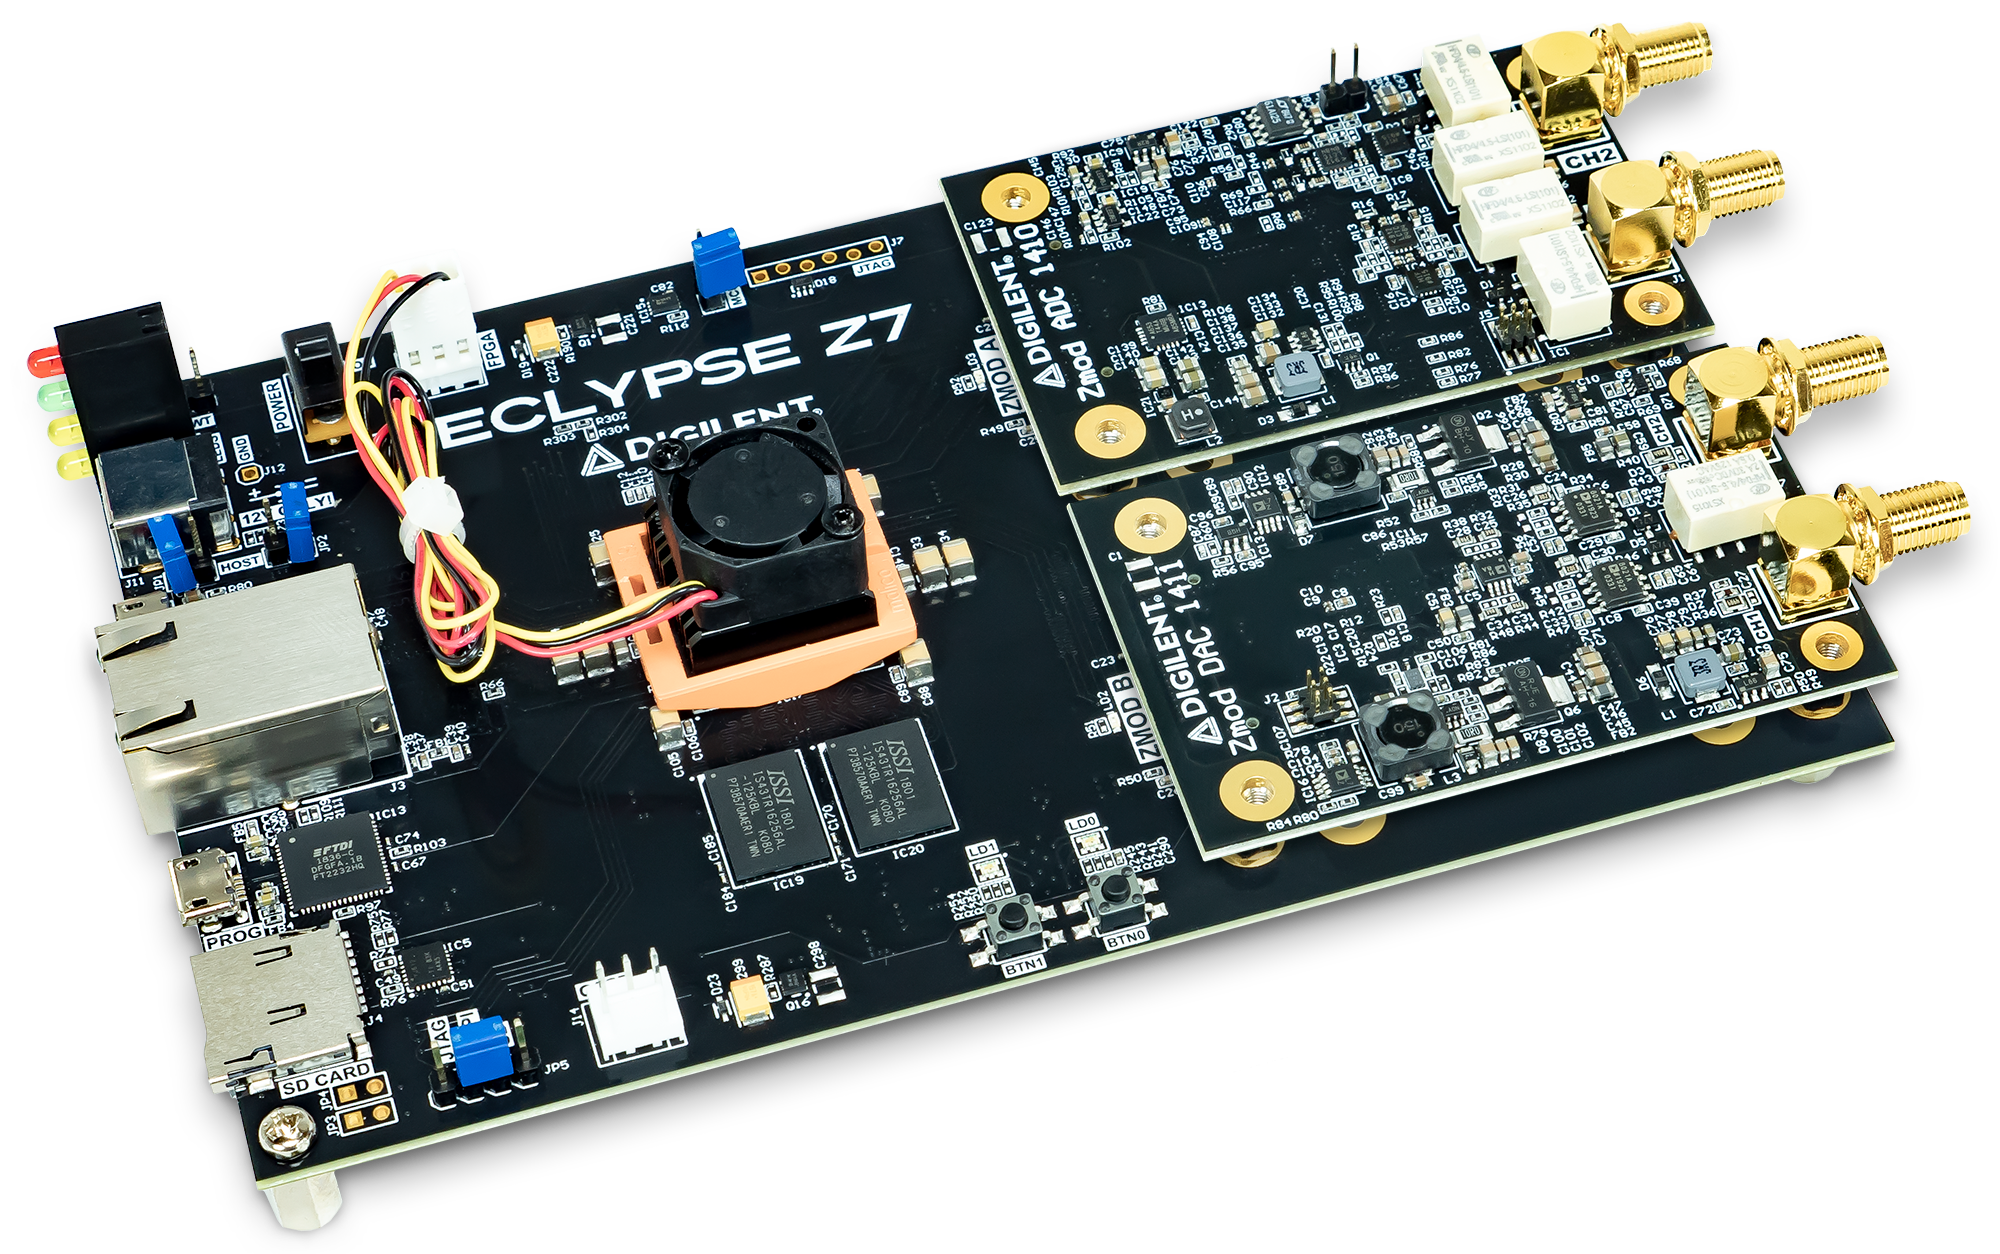
\includegraphics[width=15cm]{Eclipse-Z7}
	\caption{Bild des Eclypse-Z7 mit ADC und DAC} \faCopyright Digilent Inc. \cite{DIG_EZ7_REF}
\end{figure}

Hauptgrund für die Auswahl dieses Boards ist der, im Vergleich zu anderen FPGA Mezzanine Card (FMC) basierten Boards, relativ günstige Preis, sowie das Vorhandensein von
vielen IP-Cores der Firma Digilent welche die Ansteuerung der einzelnen Hardware-Komponenten vereinfachen und dem großen Umfang von verfügbaren Referenzmaterialien.

Der von dem Board verwendete \acs{ADC} \textit{(ZModScope 1410-105, AD9648BCPZ-105)} erfüllt alle gestellten Anforderungen.\cite{DIG_EZ7_ADC_REF}

Bei dem verwendeten \acs{FPGA} handelt es sich um einen XC7Z020-1CLG484C mit Dual-Core Cortex-A9 Prozessor mit \qty{666}{M\hertz}, sowie \qty{1}{GiB} externem DDR3-DRAM\cite{DIG_EZ7_REF}

Ein DAC wäre ebenfalls vorhanden, wird jedoch nicht genutzt.


	\chapter{Entwurf und Design}
\section{\acs{FPGA}-Design}
Nach der Festlegung der Anforderungen wurde mit der Konzeption und Entwurfsphase des gesamt Systemes sowie des \acs{FPGA}-Designs begonnen.

Hierbei wurde zuerst anhand der Anforderungen die Architektur des zu erstellenden FPGA-Designs festgelegt.

Die Kommunikation zwischen den einzelnen Modulen, besonders für den Datenaustausch, soll zum größten Teil mit einer \acs{AXI}-Stream basierten 
Schnittstelle umgesetzt werden. Für die, hauptsächlich zur Steuerung verwendete, Kommunikation zwischen \acs{FPGA}-Design und Rechenkern sollen
\acs{AXI}-Lite basierte Registerbänke verwendet werden.

In dem folgenden Entwurf nicht betrachtet werden die weiterhin notwendigen \acs{AXI}-Infrastruktur Blöcke welche, für die Kommunikation mit dem Rechenkern weiterhin noch benötigt werden,
jedoch nicht selbst umgesetzt werden. Eine Gesamtübersicht des Designs (mit \acs{AXI}-Infrastruktur) kann im Kapitel \ref{Chap:Impl} gefunden werden.

Es handelt sich um eine klassische \acs{QPSK}-Empfängerarchitektur mit direkter digitaler Abwärtsmischung.

\begin{figure}[h]
	\centering
	\begin{tikzpicture}[scale=0.85, every node/.style={scale=0.85}]
		\def\arow{7.0}
		\def\aarow{1.6}
		\def\abrow{5.5}
		\def\acrow{9.5}
		\def\adrow{12.4}
			
		\tikzset{
			basic/.style={rectangle,draw=black, top color=white,text centered},
			PLnode/.style={basic, inner sep=1em,minimum width=14cm, minimum height=5.0cm},	
			smallnode/.style={basic, inner sep=1em,minimum width=2.5cm, minimum height=1cm},
			branch/.style={fill,circle,minimum size=5pt,inner sep=0pt,outer sep=-1pt},
			sarrow/.style={->, >={latex}, line width=1.0pt},
    		carrow/.style={<->, >={latex}, dashed, line width=1.0pt}
 		}
 		
 		\node[PLnode, label=above:PL] (PL) at (\arow,1.5) {};

		% internal Nodes

 		\node[smallnode] (PL_NCO)   at (\aarow,0.9) {NCO};
	 	\node[smallnode] (PL_MIX) at (\aarow,3.1) {MIXER}; 		 
 		\node[smallnode] (PL_CIC) at (\abrow,3.1) {CIC $\downarrow 32$};
 		\node[smallnode] (PL_FIR) at (\adrow,3.1) {FIR $\downarrow 4$};
 		\node[smallnode] (PL_PID) at (\abrow,0.9) {PID};
 		\node[smallnode] (PL_PD) at  (\acrow,0.9) {Phase detector};

		% internal interconnect arrows

 		\draw[sarrow, ->] (PL_NCO.70) -- (PL_MIX.-70) node[midway,right] {$-sin$};
 		\draw[sarrow, ->] (PL_NCO.110) -- (PL_MIX.-110) node[midway,left] {$cos$};

 		\draw[sarrow, ->] (PL_MIX.7)  -- (PL_CIC.173) node[midway,above] {$I$};
 		\draw[sarrow, ->] (PL_MIX.-7) -- (PL_CIC.-173) node[midway,below] {$Q$};
	 	
	 	\draw[sarrow, ->] (PL_CIC.7)  -- ++(3.3,0) node[branch](bI){} -- (PL_FIR.173) node[near end, above] {$I$};
 		\draw[sarrow, ->] (PL_CIC.-7) -- ++(2.8,0) node[branch](bQ){} -- (PL_FIR.-173) node[near end, below] {$Q$};

 		\draw[sarrow, ->] (PL_PID.west)  -- (PL_NCO.east) node[midway,above] {$s$}; 		
 		\draw[sarrow, ->] (PL_PD.west)  -- (PL_PID.east) node[midway,above] {$e_\varphi$}; 		
 		
 		\draw[sarrow, ->] (bI)  |- ++(2.2, -1.2) |- (PL_PD.-7); 	
 		\draw[sarrow, ->] (bQ)  |- ++(2.2, -1.2) |- (PL_PD.7); 	

		% control connections
		
		\draw[carrow, <->] (PL_PD.south)  -- ++(0, -0.8) node[branch](bC0){} -- ++(5,0) node[right,text width=2cm]{Control\\(to PS)}; 
		\draw[carrow, <-] (PL_PID.south)  -- ++(0, -0.8) node[branch](bC1){} -- (bC0);
 		\draw[carrow, <-] (PL_NCO.south)  |- (bC1);
 		
 		% external connections
 		\draw[sarrow, ->] (PL_FIR.7)  -- ++(0.9,0) node[right] {$I$ (to PS)};
 		\draw[sarrow, ->] (PL_FIR.-7) -- ++(0.9,0) node[right] {$Q$};
 		\draw[sarrow, <-] (PL_MIX.west) -- ++(-0.9,0) node[left] {(from ADC)};
 		
 		% legend
 		\path ([xshift=35mm,yshift=-2mm]current bounding box.south west) node[matrix,anchor=north west,cells={nodes={font=\sffamily,anchor=west}}, draw,thick,inner sep=1pt]{
  			\draw[carrow](0,0) -- ++ (1,0); & \node{AXI-Lite};\\
  			\draw[sarrow](0,0) -- ++ (1,0); & \node{AXI-Stream};\\
 		};
	\end{tikzpicture}
	\caption{Architektur des \acs{FPGA}-Designs (ohne \acs{AXI}-Infrastruktur)}
\end{figure}

Die Hauptkomponenten des \acs{FPGA}-Designs werden in den folgenden Abschnitten noch etwas näher erklärt.

\subsection{Mischer (Mixer)}
Der Mischer hat die Aufgabe den von dem \acs{ADC} abgetasteten Datenstrom mit den, vom lokalen Oszillator erzeugten, Trägern zu multiplizieren und so das Nutzsignal in das
Basisband zu verschieben. Die besondere Schwierigkeit liegt hier dabei, dass der Mischer mit der Taktrate des \acs{ADC}s $f_{ADC}$ betrieben werden muss.

Für den Empfang von \acs{QPSK}-modulierten Daten ist es notwendig einen komplexen Mischer \textit{(sogenannter I/Q-Mischer)} zu verwenden.
Als Eingang dienen zwei vom lokalen Oszillator (\acs{NCO}) erzeugten Referenzsignale \textit{(Sinus/Kosinus)}, sowie der \acs{ADC}-Datenstrom ($x[n]$),
welche dann wie folgt Multipliziert werden: 
\begin{equation}
	I[n] = x[n]\cdot cos(2\pi\frac{f}{f_{ADC}}\cdot n) 
\end{equation}
\begin{equation}
	Q[n] = x[n]\cdot -sin(2\pi\frac{f}{f_{ADC}}\cdot n) 
\end{equation}

Es entsteht ein komplexer Datenstrom welcher dann für die weitere Verarbeitung genutzt werden kann:
\begin{equation}
	\underline{y}[n] = I[n] - j \cdot Q[n] = x[n]\cdot e^{j2\pi\frac{f}{f_{ADC}}\cdot n}
\end{equation}

Zusätzlich zu dem Signal im Basisband entsteht bei der Mischung immer auch eine Kopie des Signals bei dem doppelten der Trägerfrequenz.\cite{WPI_COSTAS}
Die nicht erwünschte Kopie wird anschließend durch die Verwendung eines Tiefpassfilters eliminiert. Diese Aufgabe übernimmt hier der \acs{CIC}-Dezimierungsfilter.

Ein- und Ausgabeschnittstellen des Mischers sollen als \acs{AXI}-Stream realisiert werden, wobei es notwendig ist jeden Taktzyklus einen neuen Datenwert
im Mischer zu verarbeiten. 

\subsection{Lokaler Oszillator (\acs{NCO})}
Der lokale Oszillator hat die Aufgabe die von dem Mischer verwendeten Referenzsignale zu erzeugen. 

Umgesetzt ist der lokale Oszillator als Numerisch gesteuerter Oszillator (\acs{NCO}). 
Die notwendige Sinus-/Kosinusignale werden hierbei durch die sogenannte direkte digitale Synthese (\acs{DDS}) erzeugt.

Dabei handelt es sich effektiv um einen Zähler (Phasen-Akkumulator, $n$-Bit breit) von welchem anschließend die untersten $m$-Bit verwendet werden
um die Ausgangsdatenwerte in einer Lookup-Tabelle nachzuschlagen.
Anhand der Schrittweite $s$ um welche der Phasen-Akkumulator jeden Taktzyklus erhöht wird lässt sich die Grundfrequenz der ausgegebenen Sinusschwingungen einstellen.

\begin{figure}[h]
	\centering
	\begin{tikzpicture}[scale=0.85, every node/.style={scale=0.85}]
		\def\arow{0.0}
		\def\brow{4.0}
		\def\crow{10.0}
			
		\tikzset{
			basic/.style={rectangle,draw=black, top color=white,text centered},
			smallnode/.style={basic, inner sep=1em,minimum width=2.5cm, minimum height=1cm},
			branch/.style={fill,circle,minimum size=5pt,inner sep=0pt,outer sep=-1pt},
			sarrow/.style={->, >={latex}, line width=1.0pt},
    		carrow/.style={<->, >={latex}, dashed},
    		buswidth/.style={decoration={ markings,
  				mark= at position 0.5 with {\node[font=\footnotesize] {/};\node[below=1pt] {\tiny #1};}
  			}, postaction={decorate}}
 		}

		% Komponenten 		
 		
 		\node[circle, draw=black, fill=white] (SUM) at (\arow,0) {$\Sigma$};	
 		\node[smallnode] (ACC) at (\brow, 0) { Phasen-Akkumulator };
 		\node[smallnode, text width=2cm] (SLUT) at (\crow, 0) { Lookup-Tabelle\\$-sin(\varphi)$ };
 		\node[smallnode, text width=2cm] (CLUT) at (\crow, -2.5cm) { Lookup-Tabelle\\$cos(\varphi)$ };

		% Interne Verbindungen

		\draw[sarrow, ->, buswidth={n}] (SUM.east) -- (ACC.west);
		\draw[sarrow, ->, buswidth={m}] (ACC.east) -- ++(0.5,0) node[branch](b0){} -- (SLUT.west);
		\draw[sarrow, -] (b0) -- ++(0,-2) node(b1){};
		\draw[sarrow, ->, buswidth={m}] (b1.north) |- (CLUT.west);
		\draw[sarrow, ->, buswidth={n}] (b0) -- ++(0,1) -- ++(-1,0) -| (SUM.north);

		% Ausgänge
		
		\draw[sarrow, <-, buswidth={n}] (SUM.west) -- ++(-1,0) node[left]{Stellwert $s$};
		\draw[sarrow, ->] (SLUT.east) -- ++(1,0) node[right, text width=3cm]{$-sin(2\pi\frac{f}{f_{ADC}}\cdot n)$};
		\draw[sarrow, ->] (CLUT.east) -- ++(1,0) node[right, text width=3cm]{$cos(2\pi\frac{f}{f_{ADC}}\cdot n)$};
 		
	\end{tikzpicture}
	\caption{Schematischer Aufbau des lokalen Oszillators.}
\end{figure}


Die Breite des Phasen-Akkumulator, die Ausgangswertbreite sowie die Anzahl der Stützpunkte der Lookup-Tabelle haben einen großen Einfluss auf die Güte der erzeugten Schwingung.
\cite{IEEE_ART_DDS}

Der Zusammenhang zwischen Frequenzstellwert $s$ und der Ausgangsfrequenz der erzeugten Sinusschwingung $\frac{f}{f_{ADC}}$ ist abhängig von der Akkumulator Bitbreite $n$:
\begin{equation}
	\frac{f}{f_{ADC}} = \frac{s}{2^n}
\end{equation}

\subsection{\acs{CIC}-Dezimierungsfilter}

\subsection{\acs{FIR}-Kompensationsfilter}
Der \acs{FIR}-Kompensationsfilter hat die Aufgabe der weiteren Abtastratenreduzierung mit der notwendigen Bandbreiten Begrenzung. 
Er wirkt zusätzlich als Kompensationsfilter für den vorgeschalteten \acs{CIC}-Filter um dessen Schwankungen der Amplitudenkennlinie in Passband zu kompensieren.

Die Filterkoeffizienten wurden mit Matlab anhand des \acs{CIC}-Filter Frequenzganges und der gewünschten Gesamtfrequenzcharakteristik ermittelt.

TODO

Aus Zeit- und Effizienzgründen soll hier der \acs{FIR}-Filter Compiler\cite{XLX_FIR} von Xilinx verwendet werden.

\subsection{Phasen-Komparator}
Der Phasen-Komperator ermittelt aus den komplexen Basisbandsignalen ($I$/$Q$) einen Phasenfehler anhand dessen die Frequenz des lokalen Oszillators später so angepasst werden soll
dass er möglichst exakt dem Oszillator des Senders folgt.

Diese Ermittlung des Phasenfehlers erfolgt anhand der in einer Costas-Loop verwendeten Technik zur Ermittlung des Phasenfehlers.\cite{WPI_COSTAS}
Abhängig von der gewählten Modulationsart (\acs{BPSK}/\acs{QPSK}) werden die folgenden Rechenschritte für die Ermittlung des Phasenfehlers genutzt:

Für \textbf{\acs{BPSK}}:
\begin{equation}
	e_\varphi = sign(I)\cdot Q
\end{equation}

Für \textbf{\acs{QPSK}}:
\begin{equation}
	e_\varphi = sign(I)*Q - sign(Q)*I
\end{equation}

Auf die genaue Herleitung dieser Zusammenhänge soll hier verzichtet werden. Eine genauere analytische Betrachtung \cite{IEEE_ART_COSTAS} könnte später für die Auslegung der Parameter
des \acs{PID}-Reglers anhand des Streckenmodelles verwendet werden.
		
\subsection{\acs{PID}-Regler}
	
Der \acs{PID}-Regler wandelt die vom Phasen-Komperator ermittelte Phasenabweichung der Empfangssymbole und den von außen vorgegebenen Soll-Frequenzpunkt 
in ein Frequenzstellsignal für den lokalen Oszillator um. Er versucht so sie Frequenz- und Phasendifferenz zwischen dem lokalen Oszillator und dem Oszillator des Senders
auszuregeln.
	
Der (im \acs{FPGA}) zeitdiskret Implementierte Regler setzt eine Übertragungsfunktion zweiter Ordnung um: $F(z)=\frac{A\cdot z^2 + B\cdot z + C}{z^2 - 1}$, deren Parameter $A,B,C$
von außen eingestellt werden sollen. Diese flexible Umsetzung des Reglers soll es ermöglichen den Regler später für unterschiedliche Anwendungsfälle einfach zur Laufzeit anpassen zu können.

Anhand der Bilinear-Transformation (Tustin-Methode) können die zeitdiskreten Reglerparameter aus den Parametern eines zeitkontinuierlich \acs{PID}-Reglers ($K,T_n,T_v$) und der Abstastfrequenz
$T_A = \frac{32}{f_{ADC}}$ abgeleitet werden:
\begin{equation}
	A = K\cdot (1 + \frac{T_A}{2\cdot T_n} + \frac{2\cdot T_v}{T_A})
\end{equation}
\begin{equation}
	B = K\cdot (\frac{T_A}{T_n} + \frac{4\cdot T_v}{T_A})
\end{equation}
\begin{equation}
	C = K\cdot (\frac{T_A}{2\cdot T_n} + \frac{2\cdot T_v}{T_A} - 1)
\end{equation}

Die Implementierung erfolgt später anhand der Differenzengleichung welche aus der Übertragungsfunktion abgeleitet werden kann: 
\begin{equation}
	y[n] = A\cdot x[n] + B\cdot x[n-1] + C\cdot x[n-2] + y[n-2]
\end{equation}	
	\chapter{Implementierung}
Nach dem Entwurf des Systems wurde mit der Implementierung begonnen.
Hierbei wurde zuerst das \acs{FPGA}-Design umgesetzt und anschließend durch Simulation verifiziert.

Nachfolgend wurde mit der Erstellung des \acs{PYNQ}-Images begonnen und erst abschließend wurde die Python-Software(Notebooks) zur Systemsteuerung umgesetzt.
Final erfolgte ein Test des Gesamtsystems durch Empfang eines, durch einen Funktionsgenerator erzeugten, Testsignales.

Die folgenden Abschnitte sollen detailliert den verwendeten Entwicklungsprozess sowie das vorgehen bei der Implementierung der einzelnen Komponenten beschreiben.

\clearpage
\section{FPGA-Design} \label{Chap:Impl}
Die Erstellung des \acs{FPGA}-Designs erfolgte in der Hardwarebeschreibungssprache \acs{VHDL}. Diese wurde aufgrund von bestehender Erfahrungen und der bekannten Syntax ausgewählt.

Als Entwicklungsumgebung für die in \acs{VHDL} geschriebenen Komponenten wurde die \textbf{Sigasi IDE}\footnote{\href{https://www.sigasi.com}{https://www.sigasi.com}} verwendet.
Hierbei handelt es sich um eine Eclipse basierte Entwicklungsumgebung, die sich (im Vergleich zu Proprietären \acs{FPGA}-Entwicklungsumgebungen) besonders durch ihre einfache Bedienung und eine schnelle Reaktionszeit auszeichnet.
\begin{figure}[h]
	\centering
	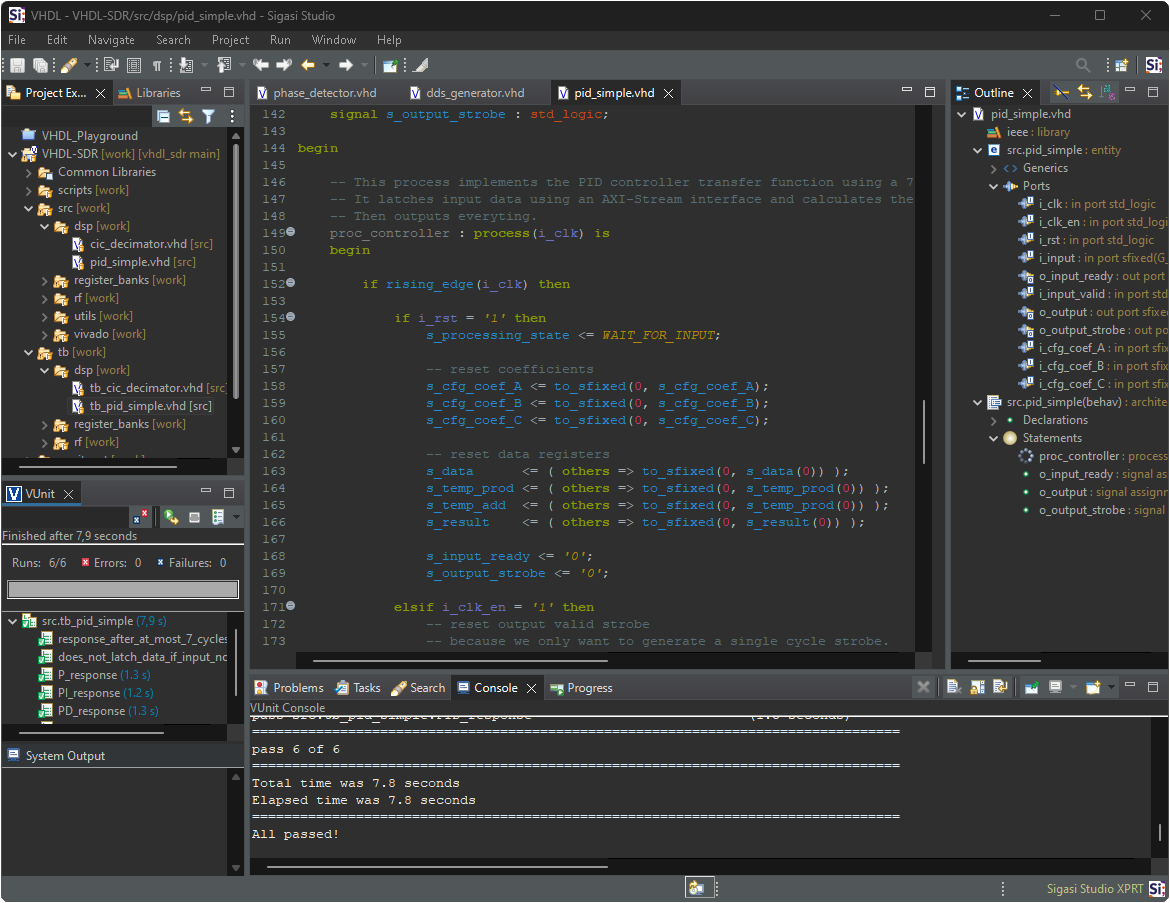
\includegraphics[width=\linewidth]{Sigasi}
	\caption{Screenshot der Sigasi IDE}
\end{figure}

Besonders Komfortabel an dieser Entwicklungsumgebung, ist die Möglichkeit externe Simulatoren (z.B. XSIM oder GHDL) sowie externe Testframeworks (z.B. OSVVM, VUnit) 
einfach integrieren zu können und so Tests direkt aus der Entwicklungsumgebung möglich machen.

Als Verifikationsframework wurde \textbf{VUnit}\footnote{\href{https://vunit.github.io}{https://vunit.github.io}} verwendet.
Hierbei handelt es sich um Open-Source Unit-Testing Framework für VHDL welches über Python angesteuert werden kann und bereits viele Verfikationskomponenten (z.B. Bus-Master) beinhaltet.

Als besonders nützlich stellte sich hier die Möglichkeit Python für die Erstellung und Verifikation von Testdaten nutzen zu können heraus.
Das hierzu angewendeten Verfahren wird näher bei der Verifikation der einzelnen Komponenten beschrieben. 

Als Simulator wurde \textbf{GHDL}\footnote{\href{http://ghdl.free.fr}{http://ghdl.free.fr}} verwendet.

Für die Synthese und OnChip-Implementierung des Designs sowie die Erstellung des Block-Designs des \acs{FPGA}-Bitstreams wurde die von Xilinx bereitgestellte Entwicklungsumgebung \textbf{Vivado} verwendet.

\subsection{Vorgehen bei der Implementierung}

Begonnen wurde die Implementierung mit der Erstellung des \acs{VHDL}-Codes.

\begin{figure}[h]
	\centering
	\begin{tikzpicture}[scale=0.85, every node/.style={scale=0.85}, node distance=2cm]
		
		\tikzstyle{startstop} = [rectangle, rounded corners, minimum width=3cm, minimum height=1cm,text centered, draw=black, fill=red!30]
		\tikzstyle{process} = [rectangle, minimum width=4.5cm, minimum height=1cm, text centered, draw=black, fill=orange!30]
		\tikzstyle{decision} = [diamond, minimum width=3cm, minimum height=1cm, text centered, draw=black, fill=green!30]
		\tikzstyle{arrow} = [thick,->,>=stealth]

		\node (start) [startstop] {Start};
		\node (impl) [process, below of=start] {Implementierung};
		\node (sim) [process, below of=impl] {Simulation};
		\node (sim_ok) [decision, below of=sim]  {OK?};

		\node (synth) [process, below of=sim_ok] {Synthese};
		\node (timing) [process, below of=synth] {Check Timing};
		\node (timing_ok) [decision, below of=timing]  {OK?};
		\node (schem) [process, below of=timing_ok] {Check Schematic};
		\node (schem_ok) [decision, below of=schem]  {OK?};
		\node (docu) [process, below of=schem_ok]  {Dokumentation};
		\node (stop) [startstop, below of=docu] {Fertig};
		
		\draw [arrow] (start) -- (impl);
		\draw [arrow] (impl) -- (sim);
		
		\draw [arrow] (sim) -- (sim_ok);
		\draw [arrow] (sim_ok.east) -- ++(2,0) node[midway, anchor=south]{Nein} |- (impl.-5);
		\draw [arrow] (sim_ok.south) -- (synth) node[midway, anchor=west]{Ja};
		
		\draw [arrow] (synth) -- (timing);
		\draw [arrow] (timing) -- (timing_ok);
		\draw [arrow] (timing_ok.east) -- ++(2.5,0) node[midway, anchor=south]{Nein} |- (impl.east);
		\draw [arrow] (timing_ok.south) -- (schem) node[midway, anchor=west]{Ja};
		
		\draw [arrow] (schem) -- (schem_ok);
		\draw [arrow] (schem_ok.east) -- ++(3,0) node[midway, anchor=south]{Nein} |- (impl.5);
		\draw [arrow] (schem_ok.south) -- (docu) node[midway, anchor=west]{Ja};

		\draw [arrow] (docu) -- (stop);

	\end{tikzpicture}
	
	\caption{Ablauf der Implementierung} \label{Abb:Impl}
\end{figure}
 
Hierbei wurden zuerst die Eingangs-/Ausgangsports der einzelnen Komponenten spezifiziert. 
Anschließend wurde die im Entwurf festgelegte Funktionalität umgesetzt. 

Wo möglich wurden funktional zusammengehörige Gruppen in eigene Komponenten ausgelagert, diese dann separat umgesetzt und dabei möglichst generisch gestaltet.

Besonderes Augenmerk lag ebenfalls auf dem effizienten Mapping von \acs{VHDL}-Code auf die einzelnen primitiven Logikelementen welche der \acs{FPGA} zur Verfügung stellt.. 
So wurde z.B. besonders Multiplikationen so umgesetzt, dass bei der späteren Synthese möglichst viele vorhandene \acs{DSP}-Slices bei der Synthese verwendet werden können.
Besonders hilfreich war hier die von Xilinx zur Verfügung gestellte Dokumentation zum Aufbau der vorhanden DSP-Slices\cite{XLX_DSP}.

Nach bzw. während der Erstellung des \acs{VHDL}-Codes wurde eine funktionelle Simulation der einzelnen Komponenten durchgeführt.
Hierbei wurden Testfälle (Testbenches) erstellt welche, soweit möglich, die Funktionalität der Komponenten bereits selbstständig verifizieren.
Dies sollte den manuelle Verifikationsaufwand gering halten und die Wiederholbarkeit der Testfälle erhöhen.
Besonders vereinfacht wurde die Testfallerstellung durch die von VUnit bereitgestellten Bibliotheken sowie der Möglichkeit externe Python-Scripte in den Testfällen zu verwenden.
Wo eine automatische Testfallüberprüfung nicht möglich wurde das Verhalten der Komponenten manuell überprüft.

Nach Durchführung der Simulation wurden die einzelnen Komponenten separat in Vivado synthetisiert.
Anhand diesen synthetisierten Designs wurden anschließend das Erreichen der gewünschten maximalen Taktrate überprüft.
Wurde diese initial nicht erreicht so wurde der \acs{VHDL}-Code durch Einführung von Zwischenregistern (Pipelining) angepasst, bis die gewünschte Taktrate erreicht wurde.

Besonders wichtig, wenn auch mühselig, war hier ebenfalls die Kontrolle des von Vivado erstellten Schaltplanes um zu überprüfen ob die gewünschten Hardware-primitiven (z.B. \acs{DSP}-slices)
richtig eingefügt werden konnten. 
Hilfreich waren hier besonders die von Vivado bereitgestellten Build-Logs aus welchen Informationen zu verwendeten primitiven gewonnen werden konnten (DSP-Utilization-Report).

Nach funktionaler Fertigstellung des \acs{VHDL}-Codes wurde abschießend Dokumentation erstellt welche die einzelnen Komponenten sowie deren interne Funktion beschreiben und erklären soll.
Die Dokumentation wurde in der Form von Inline-Code-Dokumentation erstellt.

Der hier beschriebenen Implementierungsprozess wird ebenfalls von \ref{Abb:Impl} dargestellt.

\clearpage

\subsection{Mischer (Mixer)}
Der Mischer hat die Aufgabe den vom \acs{ADC} gewonnenen Datenstrom mit den vom \acs{NCO} erzeugten Trägersignalen zu Multiplizieren.
Aufgrund der Tatsache, dass dies vor der Dezimierung des Eingangssignals erfolgt, handelt es sich hier um eine kritische Stelle. 
Deren Performance die maximale Taktrate bestimmt, mit dem das System betrieben werden kann.

Es wurde deswegen besonders darauf geachtet, den \acs{VHDL}-Code so zu gestalten, dass für die notwendigen Multiplikationen \acs{DSP}-Slices verwendet werden können.

Die Multiplikationsoperanden sowie das Ergebnis werden im Festkomma-Format dargestellt.
Das Ergebnis der Multiplikation wird auf die Bit-Breite des Eingangssignales gerundet. Die Rundungsart ist einstellbar. 

\subsection{Lokaler Oszillator (NCO)}
Die Umsetzung des lokalen Oszillators erfolgt anhand der in \ref{Sec:NCO} beschriebenen Struktur.
Da hier ebenfalls einmal pro \acs{ADC}-Taktzyklus Ausgangswerte generiert werden müssen, handelt es sich hier ebenfalls um ein Performance-kritisches Modul.

Es wurde deswegen besonders drauf geachtet, die notwendigen Sinus/Kosinus Lookup-Tabellen als Block-RAM (\acs{BRAM}) umsetzen zu können.

Für langsame Trägersignale wurde hier zusätzlich die (optionale) Möglichkeit geschaffen zwischen Stützstellen der Lookup-Tabelle linear zu interpolieren.
Diese Option bietet besonders bei geringen Trägerfrequenzen und einer geringen Anzahl von Stützstellen einen Gewinn in der Güte des Trägersignales.
Dies erfolgt jedoch auf Kosten der maximalen erreichbaren Taktfrequenzen.

Zusätzlich kann jeder Träger optional invertiert werden um etwaige Vorzeichenprobleme im Empfänger auszugleichen.

Nach \cite{IEEE_ART_DDS} wären mehrere Maßnahmen denkbar, welche die Größe der Lookup-Tabelle verringern ohne die Anzahl der Stützpunkte zu reduzieren.
Aus Einfachheit wurde hier jedoch drauf verzichtet und der Oszillator verwendet eine Lookup-Tabelle deren Größe der Anzahl der Stützpunkte entspricht.

Die unterschiedlichen Parameter des Oszillators (Akkumulatorbreite $n$, Anzahl der Stützstellen $2^m$, sowie die Bitbreite der erzeugten Träger kann über generische
Parameter während der Synthese eingestellt werden.

Die Verifikation des Oszillators erfolgte durch eine spektrale Analyse der erzeugten Träger.
Anhand des ermittelten Spektrums der erzeugten Träger wurden Position der Grundschwingung, Anteil und Amplitude der Harmonischen und die Phasenlage der Träger zueinander ermittelt.
Dies erfolgte für unterschiedliche Parameterkonfigurationen.

Die folgende Abbildung \ref{Abb:Carrier} zeigt beispielhaft das Spektrum eines erzeugten Kosinus-Trägers für eine Oszillatorfrequenz $f=\qty{14.41}{M\hertz}$ bei einer \acs{ADC}-Taktrate von $f_{ADC}=\qty{100}{M\hertz}$ einer 
Akkumulatorbreite von $n=\qty{21}{bit}$ und einer Anzahl von $1024$ Stützpunkten ($m=\qty{10}{bit}$)

\begin{figure}[h]
	\centering
	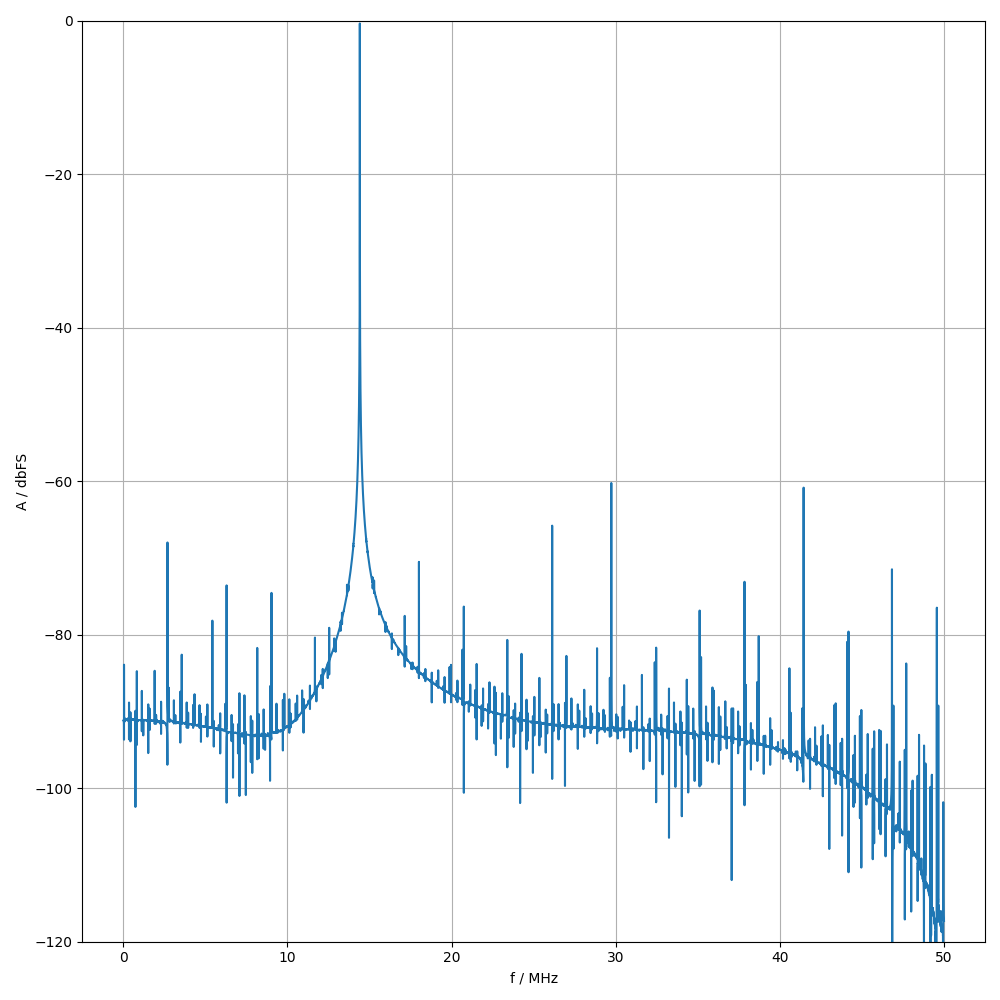
\includegraphics[width=0.8\linewidth]{spectrum_cos}
	\caption{Spektrum des $cos$ Trägers für: $f_{adc}=\qty{100}{M\hertz},f=\qty{14.41}{M\hertz}, n=21, m=10$ }
	 \label{Abb:Carrier}
\end{figure}

Die aus der Theorie erwarteten Kenngrößen\cite{IEEE_ART_DDS} konnten durch die gemessen Daten bestätigt werden.

\subsection{\acs{CIC}-Dezimerungssfilter}
Die Implementierung des \acs{CIC}-Dezimierungssfilter wurde anhand des in \ref{Sec:CIC} spezifizierten Entwurfs durchgeführt.

Soweit möglich können die Filterparameter (Ordnung $N$, Dezimierungsrate $R$) über generische Parameter während der Synthese festgelegt werden.

Um die Implementierung des Filters zu vereinfachen wurde hier jedoch bestimmte Einschränkungen der Parameter getroffen:
\begin{itemize}
	\item der Dezimierungsfaktor muss eine Zweierpotenz sein\\
	      \textit{(Dies vereinfacht die Normalisierung des Filter-Gains, da die Division durch Potenzen von Zwei durch Routing erfolgen kann)}
	\item die Filterordnung muss größer oder gleich dem Dezimierungsfaktor sein\\
		  \textit{(Notwendig um die Differenzierer, sequenziell und ohne Pipelining, umsetzen zu können)} 
\end{itemize}

Da der \acs{CIC}-Filter, vor der Dezimierung, ebenfalls Daten mit dem \acs{ADC}-Taktfrequenz verarbeitet, handelt es sich hier ebenfalls um eine Komponente mit kritischen Pfaden.
Optimierungspotential wäre hier, durch Flexibilisierung der intern verwendeten Bit-Breiten (pruned-\acs{CIC}-Filter) und folglicher Reduktion der Schaltungskomplexität, noch vorhanden.

Die Verifikation des Filters erfolgte durch Vergleich der Sprungantwort mit einer von Matlab erzeugten Referenzkurve.

\subsection{Phasen-Komparator}
Der Phasen-Komparator ermittelt anhand der im Entwurf (vergleiche \ref{Sec:PD}) beschriebenen Gleichungen die Phasenabweichung des Eingangssignals.

Da der Phasen-Komparator bereits mit dem dezimierten Eingangssignal arbeitet sind hier mehrere Taktzyklen für die Verarbeitung des Datenwerts vorhanden.
Die Durchführung der Berechnung wurde deswegen in der Form eines Zustandsautomates umgesetzt.

\begin{figure}[h]
	\centering
	\begin{circuitikz}[scale=0.7, every node/.style={scale=0.7}]
		\tikzset{flipflop DE/.style={flipflop, flipflop def={t1=D, td=EN, t6=Q, c3=1, t4=\ctikztextnot{Q}}}}
		\tikzset{
			LUT/.style={muxdemux, muxdemux def={Lh=4, Rh=4, w=5, NB=0, NR=1, NL=2}, muxdemux label={L1=A, L2=B, R1=C}},
			CTRL/.style={muxdemux, muxdemux def={Lh=4, Rh=4, w=5, NB=0, NR=1, NL=2, NT=3}, muxdemux label={L1=In\_Valid, L2=Clock, cL2=1, R1=Out\_Valid, T1=EN0, T2=EN1, T3=EN3}}
		}	
		\tikzset{
			basic/.style={rectangle,draw=black, top color=white,text centered},
			branch/.style={fill,circle,minimum size=5pt,inner sep=0pt,outer sep=-1pt},
    		buswidth/.style={decoration={ markings,
  				mark= at position 0.0 with {\node[font=\footnotesize] {/};\node[below=1pt] {\tiny #1};}
  			}, postaction={decorate}}
 		}	
		
		% Input buffer registers
		\node[flipflop DE] (REG_Q) at (0,0) {REG\_Q};
		\node[flipflop DE] (REG_I) at (0,3.5) {REG\_I};

		% Mutiply
		\node[LUT, muxdemux label={N=OP\_MUL\_Q}] (OP_Q) at (5,0) {$B\cdot sign(A)$};
		\node[LUT, muxdemux label={N=OP\_MIL\_I}] (OP_I) at (5,3.5) {$A\cdot sign(B)$};

		% Temporary Storage Registers
		\node[flipflop DE] (REG_TQ) at (9,0) {REG\_TQ};
		\node[flipflop DE] (REG_TI) at (9,3.5) {REG\_TI};

		% Adder
		\node[LUT,muxdemux label={N=OP\_ADD}] (OP_ADD) at (13,2.0) {$B - A$};


		% Output register
		\node[flipflop DE] (REG_OUT) at (17,2) {REG\_O};

		% Control block
		\node[CTRL] (CTRL) at (5,-3.5) {\acs{FSM}};

		% Inputs		
		\draw[buswidth=n] (REG_I.pin 1) -- ++(-2,0) node[left]{IN\_I};
		\draw[buswidth=n] (REG_Q.pin 1) -- ++(-2,0) node[left]{IN\_Q};

		% Input buffer to Multiply
		\draw[buswidth=n] (REG_I.pin 6) -- ++(1.5,0) node[branch](bI0){};
		\draw (bI0) -| (OP_I.lpin 1);
		\draw (bI0) |- (OP_Q.lpin 1);
		
		\draw[buswidth=n] (REG_Q.pin 6) -- ++(0.75,0) node[branch](bQ0){};
		\draw (bQ0) |- (OP_I.lpin 2);
		\draw (bQ0) |- (OP_Q.lpin 2);

		% Mutiply to Temp buffer
		\draw[buswidth=n] (OP_I.rpin 1) -| (REG_TI.pin 1);
		\draw[buswidth=n] (OP_Q.rpin 1) -| (REG_TQ.pin 1);

		% Temp Buffer to adder
		\draw[buswidth=n] (REG_TI.pin 6) -| (OP_ADD.lpin 1);
		\draw[buswidth=n] (REG_TQ.pin 6) -| (OP_ADD.lpin 2);

		% adder to output register
		\draw[buswidth=n] (OP_ADD.rpin 1) -| (REG_OUT.pin 1);

		% output
		\draw[buswidth=n] (REG_OUT.pin 6) -- ++(1,0) node[right]{$e_\varphi$};

		% Clock enable, Input
		\draw (REG_I.down) -| ++(-1.3,-3.5) node[branch](clkEnB0){};	
		\draw (clkEnB0) -- (REG_Q.down);
		\draw (clkEnB0) |- (CTRL.tpin 1);	
		
		\draw (REG_TI.down) -| ++(-1.3,-3.5) node[branch](clkEnB1){};	
		\draw (clkEnB1) -- (REG_TQ.down);
		\draw (clkEnB1) -| (CTRL.tpin 2);	
		
		\draw (CTRL.tpin 3) -| (REG_OUT.down);	

		% Input valid
		\draw (CTRL.lpin 1) -- ++(-6.5,0) node[left]{IN\_Valid};		
		
		% Output valid
		\draw (CTRL.rpin 1) -- ++(11,0) node[right]{OUT\_Valid};	
		
		% Clock
		\draw (REG_I.pin 3) -| ++(-0.75,-3.5) node[branch](clkB0){};	
		\draw (clkB0) -- (REG_Q.pin 3);		
		\draw (clkB0) -- ++(0,-4.5) node[branch](clkB1){};
		\draw (clkB1) -- ++(-1.4,0) node[left]{Clock};
		\draw (clkB1) -- ++(9,0) node[branch](clkB2){};
		\draw (clkB2) -- ++(0,4.5) node[branch](clkB3){};
		\draw (clkB3) -- (REG_TQ.pin 3);
		\draw (clkB3) |- (REG_TI.pin 3);
		\draw (clkB2) -- ++(5,0) node(clkB3){};
		\draw (clkB3.west) -| (REG_OUT.pin 3);
		\draw (CTRL.lpin 2) -| ++(-1,-1.255) node[branch]{};	
		
	\end{circuitikz}
	\caption{Vereinfachter Schaltplan des Phasen-Komparators.}
\end{figure}

Ein Zustandsautomat übernimmt hier die Erzeugung der Clock-Enable Signale welche den Datenfluss durch das Modul steuern.
Die explizite Datenflusssteuerung ist notwendig, da nicht jeden Taktzyklus gültige Daten am Eingang empfangenen werden.
Da die Ermittlung des Phasenfehlers bereits mit reduzierter Datenrate erfolgt, ist es darüber hinaus nicht notwendig jeden Taktzyklus einen Wert verarbeiten zu können.

Zwischen zwei Registern befindet sich die kombinatorische Logik welche die notwendigen arithmetischen Operationen umsetzt und so die eigentliche Datenverarbeitung übernimmt.

Die Umschaltung zwischen den Modulationsarten, im obigen Schaltplan aus Übersichtlichkeitsgründen nicht enthalten, erfolgt durch Anpassung der Differenzbildung
im Block \lstinline|OP_ADD|, für \acs{BPSK}: $C = B$, für \acs{QPSK}: $C=B-A$.

\subsection{\acs{PID}-Regler}
Der \acs{PID}-Regler implementiert die in Absatz \ref{Sec:PID} ermittelte Übertragungsfunktion.

Die Umsetzung erfolgt hier, ähnlich wie bei dem Phasen-Komparator, wieder anhand eines Zustandsautomaten der die einzelnen Rechenoperationen sequenziell abarbeitet.

Es werden dadurch mehrere Taktzyklen für die Verarbeitung eines Eingangswertes benötigt.
Da der \acs{PID}-Regler jedoch ebenfalls bereits dezimierte Signale verarbeitet stehen diese Taktzyklen zur Verfügung. 

Die einzelnen für die Berechnung notwendigen Rechenschritten wurden so umgesetzt, mit so eventuell notwendigen Wartezyklen, so das möglichst viele Operation (Multiplikationen/Additionen) in 
\acs{DSP}-Slices verlagert werden können. So ist lediglich ein mit Logikelementen umgesetzter Addierer für das Endergebnis nötig.

Die Berechnung der Reglerantwort wird intern jeweils in Festkommadarstellung und mit voller Genauigkeit durchgeführt.
Am Ende der Berechnung erfolgt eine einzelne Rundung auf das Ausgangsformat. Die Rundungsart (Runden,Abscheiden) ist hierbei einstellbar.

Die Verifikation erfolgte durch Überprüfung der Sprungantwort für unterschiedliche Werte der Reglerparameter $A,B$ und $C$.
Die hierzu verwendete Referenzsprungantwort wurde mit Matlab erzeugt.

\subsection{RF-Reciever}
Der RF-Reciever bildet das Top-Level Modul des in \acs{VHDL} erstellten Teils des \acs{FPGA}-Designs.

der RF-Reciever verschaltet Mischer, den lokalen Oszillator, die \acs{CIC}-Dezimierungsfilter für $I$ und $Q$ Datenpfad, 
den Phasen-Komparator und den \acs{PID}-Regler zu einer Phasen-Regelschleife welche die Demodulation des Eingangssignales inklusive Trägerrekonstruktion übernimmt.

Grundsätzlich erfolgt hier größtenteils nur eine Instanziierung der bereits erstellten Komponenten.
Lediglich kleinere Logikteile, welche benötigt werden um die Komponenten verschalten zu können, sind hier umgesetzt.

So ist z.B. zwischen lokalem Oszillator und \acs{PID}-Regler ein Register notwendig, welches die \acs{AXI}-Stream Schnittstelle am Ausgang des \acs{PID}-Reglers 
auf den direkten Logikeingang des Oszillators anpasst.

Zusätzlich wurde der gesamte Empfangsteil anschließend, für unterschiedlichen Parameter (Trägerfrequenzen, Signal/Rauschverhältnis), durch Simulation getestet.
Es wurde zusätzlich die empirische Einstellung des Reglers vorgenommen.

Bei der Simulation wurden, mit Python, jeweils ein modulierter Datenstrom erzeugt der, anstatt den \acs{ADC}-Daten, in das System eingespeist wurde.
Hierbei wurden Trägerfrequenz $f_c$, Signal/Rausch-Verhältnis $SNR$, Frequenzfehler des Träges $\Delta f$, und Signalamplitude $A$ variiert.
Der demodulierte Datenstrom $I/Q$ wurde anschließend mit dem gesendeten Datenstrom verglichen.

Ein Simulationsergebnis, bestehend aus demodulierten Daten in komplexer und polarer Darstellung sowie den Stellwert der Phasen-Regelschleife kann im Anhang \ref{Abb:Result} gefunden werden.

\subsection{Generische \acs{AXI}-Lite Registerbank}
Um die Erstellung der \acs{AXI}-Lite Registerbänke zu vereinfachen, wurde eine generische \acs{AXI}-Lite Registerbank erstellt.

Diese wandelt alle, auf dem \acs{AXI}-Lite Bus empfangenen Lese und Schreibtransaktionen in ein einfacheres Protokoll, welches dann zur Umsetzung von 
konkreten Registerbänken verwendet werden kann.

Auf eine genaue Analyse des \acs{AXI}-Lite Protokolls soll hier verzichtet werden.

Grundlegend lässt sich jedoch zusammenfassen, dass ein \acs{AXI}-Lite Bus aus unterschiedlichen Kanälen (Channels) besteht die jeweils über einen Ready/Valid-Handshake Nutzdaten übertragen.\\
Das \lstinline|Ready| Signal gibt hierbei an ob ein Geräte bereit ist Daten zu empfangen. Das \lstinline|Valid| Signal wird genutzt um zu Signalisieren, dass gültige Daten auf dem Bus anliegen.
Ein Transfer gilt als abgeschlossen wenn gilt: \lstinline|Ready = Valid = 1|.\cite{ARM_AXI}

\begin{figure}[h]
	\centering
	\begin{tikzpicture}[scale=0.85, every node/.style={scale=0.85}]
		\def\orow{4.0}
			
		\tikzset{
			basic/.style={rectangle,draw=black, top color=white,text centered},
			smallnode/.style={basic, inner sep=1em,minimum width=2.5cm, minimum height=2.5cm},
			branch/.style={fill,circle,minimum size=5pt,inner sep=0pt,outer sep=-1pt},
			arrow/.style={<->, >={stealth}, line width=1.0pt},
    		bus_arrow/.style={<->, >={latex}, line width=2.0pt},
    		buswidth/.style={decoration={ markings,
  				mark= at position 0.5 with {\node[font=\footnotesize] {/};\node[below=1pt] {\tiny #1};}
  			}, postaction={decorate}}
 		}

		% Komponenten 		 		
 		\node[smallnode] (READ) at (0,0) {Read \acs{FSM}};	
 		\node[smallnode] (WRITE) at (0,4) {Write \acs{FSM}};	

		% AXI-Lite 		
 		
 		\draw[bus_arrow] ($(READ.west)+(0,0.5)$)  node[above, align=right, text width=5cm, xshift=-3cm]{AXI read address channel}  -- ++(-4,0);
 		\draw[bus_arrow] ($(READ.west)+(0,-0.5)$) node[above, align=right, text width=5cm, xshift=-3cm]{AXI read data channel}  -- ++(-4,0);
 		
 		\draw[bus_arrow] ($(WRITE.west)+(0,1)$)  node[above, align=right, text width=6cm, xshift=-3.5cm]{AXI write address channel}  -- ++(-4,0);
 		\draw[bus_arrow] ($(WRITE.west)+(0,0.0)$)  node[above, align=right, text width=6cm, xshift=-3.5cm]{AXI write data channel}  -- ++(-4,0);
 		\draw[bus_arrow] ($(WRITE.west)+(0,-1)$) node[above, align=right, text width=6cm, xshift=-3.5cm]{AXI write response channel}  -- ++(-4,0);

		% Label
	
		\draw[draw=black, dashed] (-1.8,-1.8) rectangle (1.8,5.8); 	
		\node[above] at (0, 5.8) {Generische Registerbank};

		% To register driver 		
 		
 		\draw[arrow, ->, buswidth={n} ] ($(READ.east)+(0, 1.0)$) -- ++(2,0) node[right]{R\_Address};
 		\draw[arrow, <-, buswidth={32}] ($(READ.east)+(0, 0.5)$) -- ++(2,0) node[right]{R\_Data};
 		\draw[arrow, <-,              ] ($(READ.east)+(0,-1.0)$) -- ++(2,0) node[right]{R\_Result}; 		
 		
 		\draw[arrow, ->, buswidth={n} ] ($(WRITE.east)+(0, 1.00)$) -- ++(2,0) node[right]{W\_Address};
 		\draw[arrow, ->, buswidth={32}] ($(WRITE.east)+(0, 0.50)$) -- ++(2,0) node[right]{W\_Data};
 		\draw[arrow, ->               ] ($(WRITE.east)+(0,-0.50)$) -- ++(2,0) node[right]{W\_Enable};
 		\draw[arrow, <-               ] ($(WRITE.east)+(0,-1.00)$) -- ++(2,0) node[right]{W\_Result};

		% Clk
		\node[branch] (clkB0) at (-0.5,1.8){};
		\draw[arrow, ->] (clkB0) -- (READ.north  -| clkB0);
		\draw[arrow, ->] (clkB0) -- (WRITE.south -| clkB0);
		\draw[arrow, ->] (clkB0) -- ++(3.85,0) node[right]{Clock};
		\draw[arrow,  -] (clkB0) -- ++(-4.85,0);
		
		% Reset
		\node[branch] (rstB0) at (+0.5,2.2){}; 
		\draw[arrow, ->] (rstB0) -- (READ.north  -| rstB0);
		\draw[arrow, ->] (rstB0) -- (WRITE.south -| rstB0);
		\draw[arrow, ->] (rstB0) -- ++(2.85,0) node[right]{Reset};	
		\draw[arrow,  -] (rstB0) -- ++(-5.85,0);	
 		
	\end{tikzpicture}
	\caption{Schematischer Aufbau der generischen \acs{AXI}-Lite Registerbank.}
\end{figure}

Grundbestandteile der generischen Registerbank sind zwei Zustandsautomaten, wobei jeweils ein Automat die Lesezugriffe und ein Automat die Schreibzugriffe behandelt.
Die für die Transaktionen jeweils benötigten \acs{AXI}-Lite Channels werden dabei jeweils von einem der Automaten verarbeitet.

Die \enquote{Read \acs{FSM}} wandelt dabei die \acs{AXI}-Lite read data und address Kanäle in ein einfaches kombinatorisches Interface um.

Von dem untergeordneten Modul wird erwartet, dass einen \lstinline|Clock|-Zyklus nachdem eine Adresse via \lstinline|R_Address| bereitgestellt wurde
das Ergebnis der Leseoperation via \lstinline|R_Data| bereitgestellt wird.\\
\lstinline|R_Result| kann hierbei verwendet werden um ungültige Lesezugriffe abzulehnen. 

Die \enquote{Write \acs{FSM}} wandelt die \acs{AXI}-Lite write address, data und response Kanäle in ein einen synchronen write-enable basierten Bus um.

Von dem untergeordneten Modul wird hierbei erwartet, dass es bei jeder steigenden Flanke von \lstinline|Clock|, solange \lstinline|W_Enable| aktiv ist, 
die in \lstinline|W_Data| bereitgestellten Daten in das Register an der Adresse \lstinline|W_Address| speichert.\\ 
\lstinline|W_Result| kann hierbei verwendet werden um ungültige Schreibzugriffe abzulehnen. 

\subsection{Block-Design}
Das Block Design, welches gleichzeitig das Toplevel-Design des \acs{FPGA}s darstellt, wurde mit Vivado erstellt.
Hierbei wurden die in \acs{VHDL} erstellten Komponenten als \acs{RTL}-Blöcke in das Block-Design übernommen und anschließend mit den weiteren notwendigen Komponenten verbunden.

Hierbei wurden auch alle zusätzlich, für die Interaktion der \acs{RTL}-Komponenten untereinander oder mit dem Rechenkern, benötigten AXI-Infrastruktur Blöcke eingefügt.
Notwendige zusätzlich Blöcke waren:
\begin{enumerate}
	\item \textbf{\acs{AXI} \acs{DMA}-Controller}: für die Übertragung der \acs{AXI}-Stream Daten an die \acs{CPU}\cite{XLX_DMA}.
	\item \textbf{\acs{AXI}-Interconnect}: für die Verbindung der \acs{AXI}-Busse welche für Steuerregister oder die \acs{DMA}-Controller verwendet werden\cite{XLX_AXI_INT}.
	\item \textbf{\acs{AXI}-Stream FIFO/Converter}: für die Verbindung der einzelnen \acs{RTL} Module untereinander und mit dem \acs{DMA}-Controller wenn Daten umgewandelt
	oder gepuffert werden mussten\cite{XLX_AXIS}.
\end{enumerate}

Zusätzlich wurde der von Digilent bereitgestellte ZModScopeController\cite{DIG_EZ7_ADC_REF} verwendet um mit dem \acs{ADC} zu kommunizieren.

Dabei ist zu beachten, dass es bei Vivado nur möglich ist \acs{RTL}-Komponenten in das Blockdesign zu integrieren, welche in \acs{VHDL}-2000 oder 
niedriger erstellt wurden und \lstinline|std_logic| basierte Ein/Ausgänge benutzen. 

Da der Großteil des \acs{VHDL}-Codes in \acs{VHDL}-2008 erstellt wurde und zusätzlich viele selbst definierte Typen für Ein/Ausgabeports verwendet wurden, war es notwendig 
Wrapper der einzelnen Komponenten zu erstellen.
Diese abstrahieren alle nicht \lstinline|std_logic| basierte Datentypen und passten das Sprachlevel auf \acs{VHDL}-2000 an. 
Dies erfolgte üblicherweise in zwei Schritten, ein \acs{VHDL}-2008 basierter Wrapper welche alle Datentypen in \lstinline|std_logic| oder \lstinline|std_logic_vector| umwandelt.
Und anschließend ein zweiter Wrapper, welcher das Sprachniveau auf \acs{VHDL}-2000 bringt. \\
Im Quellcode wurden Wrapper nach folgendem Schema benannt:\\
 \lstinline|<name_des_moduls>_wrapper_<sprach_level>.vhd|

Eine Übersicht über das Blockdesign kann im Anhang \ref{Appendix:BlockDesign} gefunden werden.

\section{Software}

\subsection{\acs{PYNQ}-Image}
Vor der Erstellung der Software war es notwendig das \acs{PYNQ}-Image für den \acs{FPGA} zu erstellen.
Hierzu wird ein \acs{FPGA}-Design benötigt welches die Standardkonfiguration der Rechenkerne beschreibt. Als \acs{FPGA}-Design wurde das bereits erstellte Design verwendet.

Anhand des \acs{FPGA}-Designs ist es dann möglich ein \acs{PYNQ} Board-Support-Package zu erstellen. Dieses beinhaltet die gesamte Board spezifische Konfiguration.
Um dieses Board-Support-Package zu erstellen wurde die \acs{PYNQ} Dokumentation befolgt \cite{PYNQ_SD_CARD}.

Anhand des Board-Support-Packages ist es anschließend möglich das \acs{PYNQ}-Image zu erstellen.

Es wurde die Ubuntu version 22.04 verwendet, welche von \acs{PYNQ} nicht direkt unterstützt wird. 
Es war deshalb notwendig die \acs{PYNQ}-Scripte so anzupassen, dass Überprüfungen ob die korrekte Betriebssystemversion verwendet wurde auch für Ubuntu 22.04 erfolgreich waren.

Zusätzliches Hindernis war das in der verwendeten Ubuntu-Distribution standardmäßig \acs{ZFS} mit Kompression zu Einsatz kam.
Dies wird von \acs{PYNQ} nicht unterstützt und es kommt zu einem Fehler bei der Erstellung des SD-Karten Images.
Es ist deswegen notwendig die \acs{ZFS}-Kompression für den Ordner, aus dem das \acs{PYNQ}-Buildsystem aufgerufen wird, zu deaktivieren.

Nach der Erfolgreichen Erstellung des \acs{PYNQ}-Images konnte dieses auf eine SD-Karte gespielt und auf dem Board getestet werden.

\subsection{Jupyter-Notebooks}
Die Erstellung der eigentlichen und nur sehr rudimentär ausgeprägten Steuersoftware wurde anschließend über das Jupyter Webinterface vorgenommen.

Dazu wurde ein Jupyter Notebook erstellt welches:
\begin{enumerate}[label*=\arabic*.]
	\item den \acs{FPGA}-Bitstream auf den PL-Teil des \acs{FPGA}s läd
	\item die Steuerregister für \acs{ADC} und RF-Demodulator mit den korrekten Werten beschreibt
	\item den \acs{DMA}-Controller in Betrieb nimmt, so dass Daten zum Rechenkern übertragen werden können
	\item die vom \acs{DMA}-Controller empfangenen Daten anzeigt
\end{enumerate} 

Hierbei war vor allem die Dokumentation und der Quellcode der von \acs{PYNQ} bereitgestellten Python Bibliothek sehr hilfreich\cite{PYNQ_PYHTON}.

	
	
	\cleardoublepage
	\pagenumbering{Alph}	
	\thispagestyle{empty}		

	% Literaturverzeichniss
	\bibliography{references}{}

	% Abkürzungen
	% Titel des Abkürzungsverzeichnisses
\chapter*{Abkürzungsverzeichnis}
\addcontentsline{toc}{chapter}{Abkürzungsverzeichnis}\label{Sec:Abkuerzungen}

\begin{acronym}
 \acro{FPGA}{Field-programmable gate array}
 \acro{SDR}{Software defined radio}
 \acro{ADC}{Analog-to-digital converter}
 \acro{BPSK}{Binary Phase-Shift Keying}
 \acro{QPSK}{Quadratur Phase-Shift Keying}
 \acro{CPU}{Central Processing Unit}
 \acro{NCO}{Numerically Controlled Oscillator}
 \acro{AXI}{Advanced eXtensible Interface}
 \acro{DMA}{Direct Memory Access}
 \acro{APSoC}{All programmable System on a Chip}
 \acro{BRAM}{Block random access memory}
 \acro{CLB}{Configurable logic block}
 \acro{DSP}{Digital Signal Processing}
 \acro{IOB}{Input/Output-Buffer}
 \acro{DAC}{Digital-to-analog converter}
 \acro{CIC}{Cascaded-Integrator-Comb}
 \acro{FIR}{Finite impulse response}
 \acro{PID}{Propertional-Integral-Differential}
 \acro{NCO}{Numerically controlled oscillator}
 \acro{DDS}{Direct digital synthesis}
\end{acronym}	
	
	% Abbildungsverzeichnis
	\clearpage
	\addcontentsline{toc}{chapter}{Abbildungsverzeichnis}\label{Sec:Abbildungen}
	\listoffigures
	
	% Tabellenverzeichnis
	\clearpage
	\addcontentsline{toc}{chapter}{Tabellenverzeichnis}\label{Sec:Tabellen}
	\listoftables
	
\end{document}